\documentclass[12pt,letterpaper]{article}
\usepackage[utf8]{inputenc}
\usepackage{kpfonts}
\usepackage[T1]{fontenc}

% custom titles
\usepackage{titlesec}

% fix broken title numbering with 2016 titlesec update
\usepackage{etoolbox}

\makeatletter
\patchcmd{\ttlh@hang}{\parindent\z@}{\parindent\z@\leavevmode}{}{}
\patchcmd{\ttlh@hang}{\noindent}{}{}{}
\makeatother
%%%

\titlespacing*\section{0pt}{12pt plus 4pt minus 2pt}{0pt plus 2pt minus 2pt}
\titlespacing*\subsection{0pt}{12pt plus 4pt minus 2pt}{0pt plus 2pt minus 2pt}
\titlespacing*\subsubsection{0pt}{12pt plus 4pt minus 2pt}{0pt plus 2pt minus 2pt}

% Package for double spacing
\usepackage{setspace}
\usepackage{ragged2e}

% Set 1.0 inch margins
\usepackage[margin=1.0in, headheight=15pt]{geometry}
\usepackage{enumitem}

% Use images and graphics
\usepackage{graphicx}
\usepackage{float}

% Use nicer headers
\usepackage{fancyhdr}
\pagestyle{fancy}
\renewcommand{\headrulewidth}{0pt}
\rhead{CIS3750 - Lab Demo 1}

% sections should be indexed with alphabets
\renewcommand{\thesection}{\Alph{section}}

%double spaced lines in the whole document
\doublespacing

\title{Assignment 1}

\begin{document}
\begin{titlepage}
    \centering
    \vspace*{\baselineskip}
    \rule{\textwidth}{1.6pt}\vspace*{-\baselineskip}\vspace*{2pt}
    \rule{\textwidth}{0.4pt}\\[1.5\baselineskip]
    {\LARGE \textsc{Reflections on a Paper Prototyping Session}}\\[\baselineskip]
	\rule{\textwidth}{0.4pt}\vspace*{-\baselineskip}\vspace{4pt}    
    \rule{\textwidth}{2pt}\\[2\baselineskip]
   
    \vspace*{5\baselineskip}
    \textsc{BY}\\[0.25\baselineskip]
    {\LARGE HANLON} \\
    
    \vspace*{\baselineskip}
    % List of authors in alphabetical order (by last name)
    {\textsc{David DiMaria \\ Braydon Johnson \\ Joshua Lemieux \\ Neivin Mathew \\ Like Zheng} \par}
    \vfill
    {\scshape October 14, 2016} \\
  \end{titlepage}
  
  
% Table of Contents (no page numbers on contents)
\pagenumbering{roman} %roman numerals for ToC
\tableofcontents
\lhead{} % remove default header from Contents page
\clearpage
\pagenumbering{arabic} %pagenumbering in arabic numbers
    
\clearpage
\section{Team Details}
\subsection{Team Name}
The team name for the project is "Hanlon."\par
The name is inspired by the eponymous highway that runs through the city of Guelph, and signifies the team's ties to the University of Guelph, and its beautiful city.\\

\begin{figure}[H]
	\centering	
	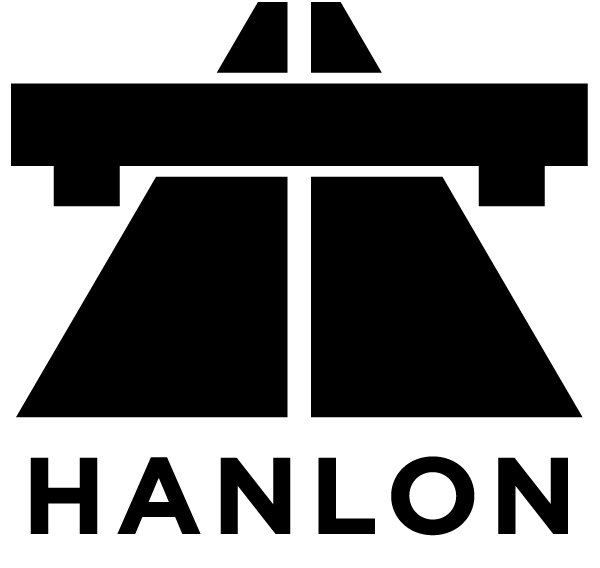
\includegraphics[height=2in]{img/hanlon-logo.png}
	%\caption{The team logo}
	\label{fig:kitten}
\end{figure}

\subsection{Team Members}
Hanlon is comprised of the following students:\\
1. \textbf{\hspace*{8pt}David DiMaria} - Project Manager\\
2. \textbf{\hspace*{8pt}Braydon Johnson} - Software Developer, User Interface Designer\\
3. \textbf{\hspace*{8pt}Joshua Lemieux} - Project Manager, User Interface Designer\\
4. \textbf{\hspace*{8pt}Neivin Mathew} - Software Developer, User Interface Designer\\
5. \textbf{\hspace*{8pt}Like Zheng} - Software Developer

\subsection{Team Roles}
\subsubsection*{Project Manager}
The Project Manager predicts potential problems that may arise during development, and plans tasks to ensure that the project is completed successfully and on time. This role involves the scheduling and unblocking of tasks. It may also involve some programming.

\subsubsection*{Software Developer}
The Developer is involved in all aspects of the software development process including research, design, coding, documentation and testing.

\subsubsection*{User Interface Designer}
The User Interface (UI) Designer role is to plan out and develop any user facing component of the system which includes the specific layout of screens, and improving the interaction between the customer and the product.

\subsection{Team Organization}
Hanlon will follow a static team structure. Each member will maintain their respective roles for the entire duration of the project. \par

Hanlon will use a democratic majority voting system for any decisions that need to be taken within the team. Each present member will be involved in voting, and possesses one vote per motion. A motion is passed when a simple majority is achieved. \par

In the event of a team member being unavailable, and a majority cannot be established, a motion can only be passed through unanimous consent.

\clearpage
\section{Use Cases}
\subsection{List of Use Cases}
Participants of the Paper Prototyping session were presented with the following use cases:\\
1.\hspace*{8pt} Create a Farmer user account\\
2.\hspace*{8pt} Login to a Farmer user account\\
3.\hspace*{8pt} Answer an ARET Survey
4.\hspace*{8pt} Download a Research Article on Tomatoes\\
5.\hspace*{8pt} Add Tomatoes to your list of Crops\\
6.\hspace*{8pt} Harvest Tomatoes from your list of Crops\\
7.\hspace*{8pt} Delete Tomatoes from your list of Crops\\
8.\hspace*{8pt} Change your name in your User Profile\\
9.\hspace*{8pt} Change your Account Password\\
10.\hspace*{3pt} Log out of your Farmer user account

\subsection{Team Roles}
The members of Hanlon were responsible for different aspects of the prototyping session:\\
1. \textbf{\hspace*{8pt}David DiMaria} - Facilitator\\
2. \textbf{\hspace*{8pt}Braydon Johnson} - Observer/Note Taker\\
3. \textbf{\hspace*{8pt}Joshua Lemieux} - Human Computer\\
4. \textbf{\hspace*{8pt}Neivin Mathew} - Observer/Note Taker\\
5. \textbf{\hspace*{8pt}Like Zheng} - Observer/Note Taker
\subsection{Participants}
The prototyping session included the following four participants:\\
1.\hspace*{8pt} \textbf{Corey Alexander}\\
The participant appeared to be in their late twenties, did not seem to be able to remember some instructions, but still seemed to be familiar with mobile interfaces and possessed a moderate proficiency with computers. This participant is not very representative of the client.\\[0.5\baselineskip]
2.\hspace*{8pt} \textbf{Dominic Gagne}\\
The participant appeared to be in their mid twenties, and was very comfortable with the mobile interface and other aspects of the application. The participant is certainly highly skilled in the use of computers and is also not an accurate representation of the client.\\[0.5\baselineskip]
3.\hspace*{8pt} \textbf{Oliver Cook}\\
The participant appeared to be in their mid twenties, and was very comfortable while navigating the mobile application interface. The participant is almost certainly highly skilled in the use of computers and is also not an accurate representation of the client.\\[0.5\baselineskip]
4.\hspace*{8pt} \textbf{Katherine McRoberts}\\
The participant appeared to be in their late thirties, and seemed unfamiliar with mobile application interfaces and design standards. The participant is most likely not highly skilled in the use of computers and is quite representative of the application's target audience.
 

\clearpage
\section{Things That Worked}
It was difficult to evaluate exactly what elements of our design worked well since participants would not notice things that were as they expected. Thus, we can assume that any element of the design that the participants did not have trouble with was well designed and behaved in a way that was expected. However, some participants did have highly positive comments about certain parts of the prototype.\par
All participants thought that the process of login, and account creation went exactly as they expected. They felt that the process was straightforward, and agreed that the flow was intuitive. Upon reaching the home screen, all participants were able to recognize the menu bar at the bottom of their screen and identified it as the primary means of navigating through the application.\par
The process of adding new crops to the list of the user's currently growing crops seemed to be well received by all the participants. Most participants felt the add button occupied the same section of the screen that they expected it to be in and were able to successfully search for a new crop and add it to their growing crops without any hassles.\par
All participants agreed that new surveys available to them on their home screen were appropriately positioned and visible enough to catch their attention without being obtrusive to other application functionality.\par
Most participants were able to easy navigate through their user profile page. They were able to successfully change their name, and account password without any confusion. Most participants were also able to quickly find the logout option on the profile screen when asked to do so, and also completed the use case without any hindrance.

\clearpage
\section{Things to Improve}
Although most participants were able to easily navigate through the system without much trouble, there were some aspects of the design that were found wanting.\par
The most common complaint was about our navigation bar at the bottom of the screen. All participants felt that the icons used to indicate each screen were rather ambiguous. They felt like they did not know which screen each button would lead them to. After the first two participants had completed the prototyping session, the team decided to add text below the icons to indicate which screen each button would lead the user to. While this approach certainly helped the following participants to navigate through the application better, it had a negative impact on the overall look and feel of the application. A more permanent solution would be to overhaul the icon design and choose icons that are more representative of the screens they lead to.\par
The location of the add button on the Crops page was troublesome to one of the participants, due to the fact that they were accustomed to the iOS user experience, while our prototype followed the Android design guidelines. The user expected the add button at the top right portion of the screen, rather than the bottom right. However, it is possible that this participant is an outlier. The team believed that the position of the button was consistent with Android design patterns, which is the operating system that the majority of the user base is expected to use.\par
Participants were generally unsure as to which specific screen they were on when managing their currently grown crops. The page titles for the screens on which participants viewed their own crops and searched for new crops to add were too similar, which possibly led to the confusion. Giving each screen more descriptive titles would help alleviate the uncertainty that the participants had. Appropriate prompts to the user in search bars and other pop-up windows would also help the user understand the current state of the application.\par
Some participants wished to decline answering the survey presented to them, but had no option to do so. However, the user must have the power to be able to refuse to answer surveys that they do not wish to answer for any reason. Another issue was that the team had not accounted for how multiple surveys would present themselves to the user. To rectify these issues, the survey can have an additional decline button next to the choice to answer the survey. Additionally, multiple surveys could be presented as a collapsible list, where users can select which ones they want to answer and which ones they do not. The list can be collapsed to preserve screen real estate and be unobtrusive to user.\par
Our first participant successfully downloaded the research article, but was not provided with any feedback indicating whether the download was successful or not. Thus, the user did not have any information as to whether the application had done what they had wanted it to do or not. The team added a pop-up notification after the first session which informed the user of the status of their download, which successfully resolved the issue and would be included in the final design.

\clearpage
\section{Looking to the Future}
Throughout the prototyping session, the participants made a number of suggestions about improvements that they would like to see to some features of the application. Some also wished that there were additional features for certain parts of the application.\par
Some users felt a bit lost with all the different screens that were available to them and wished that there was something to guide them within the application itself. The addition of a tutorial section which would execute for the first run of the application would resolve this issue and would not be difficult to maintain or implement. It would also vastly improve the usability of the application.\par
A common request was the improvement of the accessibility of the application for use by the disabled. The application could certainly have accommodations for some disabilities like colour blindness, deafness, etc. which are relatively common and easy to account for. However, it is simply not practical to account for some other disabilities, as it would increase the overhead for the project. The target user of the application is a farmer, who are assumed to be able bodied individuals and increasing the size and processing power demands of our application would be unfeasible, since we must account for a variety of devices and minimize the application's footprint on the user's device.\par
When the participants were attempting to complete the use case where they harvested a crop, some tried entering very large numbers for their yields. They suggested that the application should attempt to validate these fields before approving the changes. Since all the information is provided by the user themselves, it becomes very difficult to validate any of the information, if the initial amounts are invalid as well. There is no way to know what is a valid input for something that has such a high degree of variation across different users and times. From an extensibility standpoint, catching errors like these are nigh impossible. One method that would ensure some degree of validity, is to ensure that the harvested amount is less than or equal to the initial amount planted.\par
Some users wished that there was a better way to sort the research articles displayed within the research section of the application. They felt that simply searching for keywords within articles was not enough and wanted a way to browse through the articles without knowing what they were looking for. Adding functionality to browse through research articles by date, tags, category, author, or crop would help resolve this need. Allowing users to see what research articles have been viewed the most or used the most would also help them choose which article would be helpful to them. This functionality would not be difficult to implement as it would require fetching slightly more specific data and would also be straightforward to maintain.\par
One of the participants requested for background images and music in the application. While this could potentially improve the aesthetic of the application, it would not conform with the application's design standards and would also increase the size, and processing power demands of the application. Since we are under tight mobile data constraints, and are attempting to cater a wide range of devices, some of which may have less power, this change would have adverse effects on our application and user experience. It would also require rigorous maintenance to ensure that the images and music display and play well across various devices and operating system versions. 

\clearpage
\section{Individual Contributions}
\subsection{David DiMaria}
\textbf{Yes! And... Using Improv}\par


\clearpage
\subsection{Braydon Johnson}
\textbf{The Yes! And... Philosophy}\par


\clearpage
\subsection{Josh Lemieux}
\textbf{Improvising in Business}\par


\clearpage
\subsection{Neivin Mathew}
\textbf{Improving communication with Improv}\par

		
	
\clearpage
\subsection{Like Zheng}
\textbf{Yes!And... Philosophy}\par



\clearpage
\section{References}
\begin{flushleft}
\begin{itemize}[leftmargin=12pt]

\item World Food Programme (2016). \emph{Malawi.}
 Retrieved from \texttt{https://www.wfp.org/countries/malawi}

\item Agricultural Research and Extension Trust of Malawi (2016). \emph{About ARET Malawi.}
Retrieved from \texttt{http://www.aret.org.mw/index.php/about-us/profile}

\item Agricultural Research and Extension Trust of Malawi (2016, January). \emph{ARET Strategic Plan 2016-2021.}


\end{itemize}
\end{flushleft}   



\end{document}